% ═══════════════════════════════════════════════════════════════════════════════
% richtungsfeld_fallschirmspringer.tex
%
% Richtungsfeld der ODE  v̇ = g − kv  mit k = 0,2 s⁻¹, g = 9,81 m/s²
%
% Enthält:
%   • Richtungsfeld (normierte Pfeile auf einem Gitter)
%   • Nullisokline  v = v∞ = 49,05 m/s  (orange, gestrichelt)
%   • Drei Lösungskurven für v(0) ∈ {0, 30, 70} m/s  (dunkelblau)
%
% Kompilierung:  lualatex  oder  pdflatex  (standalone → PDF)
% SVG-Export:    dvisvgm --pdf richtungsfeld_fallschirmspringer.pdf
%                         -o  richtungsfeld_fallschirmspringer.svg
% ═══════════════════════════════════════════════════════════════════════════════

\documentclass[tikz, border=6pt]{standalone}
\usepackage{pgfplots}
\pgfplotsset{compat=1.18}
\usepackage{xcolor}

% ── Farbdefinitionen (konsistent mit der TikZ- und Svelte-Palette) ────────────
\definecolor{myblue}{HTML}{005a94}      % Lösungskurven
\definecolor{myorange}{HTML}{e87846}    % Nullisokline / Grenzgeschwindigkeit

\begin{document}

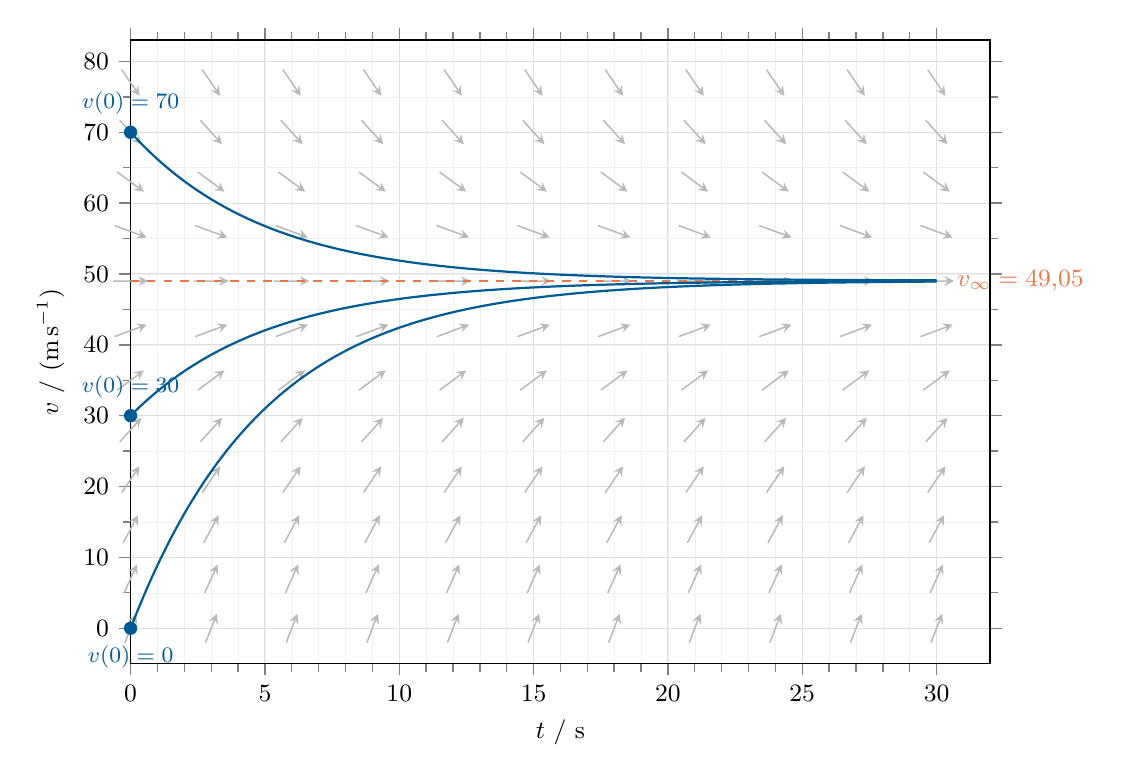
\begin{tikzpicture}

  % ── Skalierungskonstanten für die Pfeillängen-Normierung ──────────────────
  %
  % Ziel: Alle Pfeile haben dieselbe visuelle Länge L_half (in cm) im Bild.
  % Plotfläche ca. W = 9,8 cm (x: 0–32) und H = 8,2 cm (y: −5–83).
  %   sx = 9,8/32 ≈ 0,306 cm/Einheit,  sy = 8,2/88 ≈ 0,093 cm/Einheit
  % Halbe Datenlänge des Pfeils:
  %   dt = L_half / sqrt(sx² + sy²·f²),   dv = f·dt
  %
  \pgfmathsetmacro{\sxsq}{0.09364}   % sx² ≈ 0,306²
  \pgfmathsetmacro{\sysq}{0.008649}  % sy² ≈ 0,093²
  \pgfmathsetmacro{\Lhalf}{0.20}     % halbe visuelle Pfeillänge [cm]

  \begin{axis}[
    width        = 12.5cm,
    height       = 9.5cm,
    xmin = 0,    xmax = 32,
    ymin = -5,   ymax = 83,
    xlabel       = {$t$ / s},
    ylabel       = {$v$ / (m\,s$^{-1}$)},
    xtick        = {0, 5, ..., 30},
    ytick        = {0, 10, ..., 80},
    minor xtick  = {0, 1, ..., 30},
    minor ytick  = {0, 5, ..., 80},
    grid         = both,
    major grid style = {line width=0.35pt, draw=gray!25},
    minor grid style = {line width=0.20pt, draw=gray!12},
    axis line style  = {line width=0.6pt},
    tick style       = {line width=0.5pt},
    tick align       = outside,
    font             = \small,
    clip             = false,
  ]

  % ─────────────────────────────────────────────────────────────────────────
  % Richtungsfeld
  % Gitterpunkte: t ∈ {0, 3, 6, …, 30},  v ∈ {0, 7, 14, …, 77}
  % Steigung: f(v) = 9,81 − 0,2·v  (hängt nicht von t ab)
  %
  % Technik: \edef expandiert \xlo/\ylo/\xhi/\yhi vollständig zu Zahlen,
  % bevor pgfplots die Koordinaten parst. Damit entfällt die Notwendigkeit,
  % axis cs: mit Makro-Argumenten zu verwenden.
  % ─────────────────────────────────────────────────────────────────────────
  \foreach \tval in {0, 3, ..., 30} {
    \foreach \vval in {0, 7, ..., 77} {
      \pgfmathsetmacro{\f}{9.81 - 0.2*\vval}
      \pgfmathsetmacro{\denom}{sqrt(\sxsq + \sysq*\f*\f)}
      \pgfmathsetmacro{\dtt}{\Lhalf/\denom}
      \pgfmathsetmacro{\dvv}{\f*\Lhalf/\denom}
      \pgfmathsetmacro{\xlo}{\tval - \dtt}
      \pgfmathsetmacro{\xhi}{\tval + \dtt}
      \pgfmathsetmacro{\ylo}{\vval - \dvv}
      \pgfmathsetmacro{\yhi}{\vval + \dvv}
      \edef\arrowplot{%
        \noexpand\addplot[%
          gray!55, line width=0.55pt, -stealth, mark=none, forget plot%
        ] coordinates {(\xlo,\ylo)(\xhi,\yhi)};%
      }%
      \arrowplot
    }
  }

  % ─────────────────────────────────────────────────────────────────────────
  % Nullisokline  v = v∞ = g/k = 49,05 m/s  (orange, gestrichelt)
  % ─────────────────────────────────────────────────────────────────────────
  \addplot[myorange, dashed, thick, domain=0:30, samples=2, forget plot]
    {49.05};
  \node[myorange, anchor=west, font=\small\itshape]
    at (axis cs:30.4, 49.05) {$v_{\infty} = 49{,}05$};

  % ─────────────────────────────────────────────────────────────────────────
  % Lösungskurven  v(t) = v∞ + C·e^{−0,2 t},  C = v(0) − v∞
  % ─────────────────────────────────────────────────────────────────────────

  % v(0) = 0  →  C = −49,05
  \addplot[myblue, thick, domain=0:30, samples=200, forget plot]
    {49.05*(1 - exp(-0.2*x))};
  \addplot[myblue, only marks, mark=*, mark size=2.2pt, forget plot]
    coordinates {(0, 0)};
  \node[myblue, anchor=north, font=\footnotesize, yshift=-3pt]
    at (axis cs:0, 0) {$v(0)=0$};

  % v(0) = 30  →  C = −19,05
  \addplot[myblue, thick, domain=0:30, samples=200, forget plot]
    {49.05 - 19.05*exp(-0.2*x)};
  \addplot[myblue, only marks, mark=*, mark size=2.2pt, forget plot]
    coordinates {(0, 30)};
  \node[myblue, anchor=south, font=\footnotesize, yshift=3pt]
    at (axis cs:0, 30) {$v(0)=30$};

  % v(0) = 70  →  C = +20,95
  \addplot[myblue, thick, domain=0:30, samples=200, forget plot]
    {49.05 + 20.95*exp(-0.2*x)};
  \addplot[myblue, only marks, mark=*, mark size=2.2pt, forget plot]
    coordinates {(0, 70)};
  \node[myblue, anchor=south, font=\footnotesize, yshift=3pt]
    at (axis cs:0, 70) {$v(0)=70$};

  \end{axis}

\end{tikzpicture}

\end{document}
